\documentclass[a4paper]{article}

\usepackage{inputenc}
\usepackage[british,UKenglish]{babel}
\usepackage{amsmath}
%\usepackage{titlesec}
\usepackage{color}
\usepackage{graphicx}
\usepackage{fancyref}
\usepackage{hyperref}
\usepackage{float}
\usepackage{scrextend}
\usepackage{setspace}
\usepackage{xargs}
\usepackage{multicol}
\usepackage{nameref}

\usepackage{sectsty}
\usepackage{multicol}
\usepackage{multirow}
\usepackage[procnames]{listings}
\usepackage{appendix}

\newcommand\tab[1][1cm]{\hspace*{#1}}
\hypersetup{colorlinks=true, linkcolor=black}
\interfootnotelinepenalty=10000

\newcommand{\cleancode}[1]{\begin{addmargin}[3em]{3em}\texttt{\textcolor{cleanOrange}{#1}}\end{addmargin}}
\newcommand{\cleanstyle}[1]{\text{\textcolor{cleanOrange}{\texttt{#1}}}}


\usepackage[colorinlistoftodos,prependcaption,textsize=footnotesize]{todonotes}
\newcommandx{\commred}[2][1=]{\textcolor{Red}
{\todo[linecolor=red,backgroundcolor=red!25,bordercolor=red,#1]{#2}}}
\newcommandx{\commblue}[2][1=]{\textcolor{Blue}
{\todo[linecolor=blue,backgroundcolor=blue!25,bordercolor=blue,#1]{#2}}}
\newcommandx{\commgreen}[2][1=]{\textcolor{OliveGreen}{\todo[linecolor=OliveGreen,backgroundcolor=OliveGreen!25,bordercolor=OliveGreen,#1]{#2}}}
\newcommandx{\commpurp}[2][1=]{\textcolor{Plum}{\todo[linecolor=Plum,backgroundcolor=Plum!25,bordercolor=Plum,#1]{#2}}}

\def\code#1{{\tt #1}}

\def\note#1{\noindent{\bf [Note: #1]}}

\makeatletter
%% The "\@seccntformat" command is an auxiliary command
%% (see pp. 26f. of 'The LaTeX Companion,' 2nd. ed.)
\def\@seccntformat#1{\@ifundefined{#1@cntformat}%
   {\csname the#1\endcsname\quad}  % default
   {\csname #1@cntformat\endcsname}% enable individual control
}
\let\oldappendix\appendix %% save current definition of \appendix
\renewcommand\appendix{%
    \oldappendix
    \newcommand{\section@cntformat}{\appendixname~\thesection\quad}
}
\makeatother


% "define" Scala
\usepackage[T1]{fontenc}  
\usepackage[scaled=0.82]{beramono}  
\usepackage{microtype} 

\sbox0{\small\ttfamily A}
\edef\mybasewidth{\the\wd0 }

\lstdefinelanguage{scala}{
  morekeywords={abstract,case,catch,class,def,%
    do,else,extends,false,final,finally,%
    for,if,implicit,import,match,mixin,%
    new,null,object,override,package,%
    private,protected,requires,return,sealed,%
    super,this,throw,trait,true,try,%
    type,val,var,while,with,yield},
  sensitive=true,
  morecomment=[l]{//},
  morecomment=[n]{/*}{*/},
  morestring=[b]",
  morestring=[b]',
  morestring=[b]"""
}

\usepackage{color}
\definecolor{dkgreen}{rgb}{0,0.6,0}
\definecolor{gray}{rgb}{0.5,0.5,0.5}
\definecolor{mauve}{rgb}{0.58,0,0.82}

% Default settings for code listings
\lstset{frame=tb,
  language=scala,
  aboveskip=3mm,
  belowskip=3mm,
  showstringspaces=false,
  columns=fixed, % basewidth=\mybasewidth,
  basicstyle={\small\ttfamily},
  numbers=none,
  numberstyle=\footnotesize\color{gray},
  % identifierstyle=\color{red},
  keywordstyle=\color{blue},
  commentstyle=\color{dkgreen},
  stringstyle=\color{mauve},
  frame=single,
  breaklines=true,
  breakatwhitespace=true,
  procnamekeys={def, val, var, class, trait, object, extends},
  procnamestyle=\ttfamily\color{red},
  tabsize=2
}

\lstnewenvironment{scala}[1][]
{\lstset{language=scala,#1}}
{}
\lstnewenvironment{cpp}[1][]
{\lstset{language=C++,#1}}
{}
\lstnewenvironment{bash}[1][]
{\lstset{language=bash,#1}}
{}
\lstnewenvironment{verilog}[1][]
{\lstset{language=verilog,#1}}
{}



%代码段设置
\lstset{numbers=left,
basicstyle=\tiny,
numberstyle=\tiny,
keywordstyle=\color{blue!70},
commentstyle=\color{red!50!green!50!blue!50},
frame=single, rulesepcolor=\color{red!20!green!20!blue!20},
escapeinside=``
}

\graphicspath{ {figures/} }
\usepackage{ctex}
\usepackage{graphicx}
\usepackage{color,framed}%文本框
\usepackage{listings}
\usepackage{caption}
\usepackage{amssymb}
\usepackage{enumerate}
\usepackage{xcolor}
\usepackage{bm} 
\usepackage{lastpage}%获得总页数
\usepackage{fancyhdr}
\usepackage{tabularx}  
\usepackage{geometry}
\usepackage{minted}
\usepackage{graphics}
\usepackage{subfigure}
\usepackage{float}
\usepackage{pdfpages}
\usepackage{pgfplots}
\pgfplotsset{width=10cm,compat=1.9}
\usepackage{multirow}
\usepackage{footnote}
\usepackage{booktabs}

%-----------------------伪代码------------------
\usepackage{algorithm}  
\usepackage{algorithmicx}  
\usepackage{algpseudocode}  
\floatname{algorithm}{Algorithm}  
\renewcommand{\algorithmicrequire}{\textbf{Input:}}  
\renewcommand{\algorithmicensure}{\textbf{Output:}} 
\usepackage{lipsum}  
\makeatletter
\newenvironment{breakablealgorithm}
  {% \begin{breakablealgorithm}
  \begin{center}
     \refstepcounter{algorithm}% New algorithm
     \hrule height.8pt depth0pt \kern2pt% \@fs@pre for \@fs@ruled
     \renewcommand{\caption}[2][\relax]{% Make a new \caption
      {\raggedright\textbf{\ALG@name~\thealgorithm} ##2\par}%
      \ifx\relax##1\relax % #1 is \relax
         \addcontentsline{loa}{algorithm}{\protect\numberline{\thealgorithm}##2}%
      \else % #1 is not \relax
         \addcontentsline{loa}{algorithm}{\protect\numberline{\thealgorithm}##1}%
      \fi
      \kern2pt\hrule\kern2pt
     }
  }{% \end{breakablealgorithm}
     \kern2pt\hrule\relax% \@fs@post for \@fs@ruled
  \end{center}
  }
\makeatother
%------------------------代码-------------------
\usepackage{xcolor} 
\usepackage{listings} 
\lstset{ 
breaklines,%自动换行
basicstyle=\small,
escapeinside=``,
keywordstyle=\color{ blue!70} \bfseries,
commentstyle=\color{red!50!green!50!blue!50},% 
stringstyle=\ttfamily,% 
extendedchars=false,% 
linewidth=\textwidth,% 
numbers=left,% 
numberstyle=\tiny \color{blue!50},% 
frame=trbl% 
rulesepcolor= \color{ red!20!green!20!blue!20} 
}

%-------------------------页面边距--------------
\geometry{a4paper,left=2.3cm,right=2.3cm,top=2.7cm,bottom=2.7cm}
%-------------------------页眉页脚--------------
\usepackage{fancyhdr}
\pagestyle{fancy}
\lhead{\kaishu \leftmark}
% \chead{}
\rhead{\kaishu 并行程序设计实验报告}%加粗\bfseries 
\lfoot{}
\cfoot{\thepage}
\rfoot{}
\renewcommand{\headrulewidth}{0.1pt}  
\renewcommand{\footrulewidth}{0pt}%去掉横线
\newcommand{\HRule}{\rule{\linewidth}{0.5mm}}%标题横线
\newcommand{\HRulegrossa}{\rule{\linewidth}{1.2mm}}
\setlength{\textfloatsep}{10mm}%设置图片的前后间距
%--------------------文档内容--------------------

\begin{document}
\renewcommand{\contentsname}{目\ 录}
\renewcommand{\appendixname}{附录}
\renewcommand{\appendixpagename}{附录}
\renewcommand{\refname}{参考文献}
\renewcommand{\figurename}{图}
\renewcommand{\tablename}{表}
\renewcommand{\today}{\number\year 年 \number\month 月 \number\day 日}

%-------------------------封面----------------
\begin{titlepage}
  \begin{center}
    
\includegraphics[width=0.8\textwidth]{NKU.png}\\[1cm]
    \vspace{20mm}
    \textbf{\huge\textbf{\kaishu{计算机学院}}}\\[0.5cm]
    \textbf{\huge{\kaishu{并行程序设计第一次作业}}}\\[2.3cm]
    \textbf{\Huge\textbf{\kaishu{Apple M1体系架构调研}}}

    \vspace{\fill}

    % \textbf{\Large \textbf{并行程序设计期末实验报告}}\\[0.8cm]
    % \HRule \\[0.9cm]
    % \HRule \\[2.0cm]
    \centering
    \textsc{\LARGE \kaishu{姓名\ :\ 丁屹}}\\[0.5cm]
    \textsc{\LARGE \kaishu{学号\ :\ 2013280}}\\[0.5cm]
    \textsc{\LARGE \kaishu{专业\ :\ 计算机科学与技术}}\\[0.5cm]

    \vfill
    {\Large \today}
  \end{center}
\end{titlepage}

\renewcommand {\thefigure}{\thesection{}.\arabic{figure}}%图片按章标号
\renewcommand{\figurename}{图}
\renewcommand{\contentsname}{目录}
\cfoot{\thepage\ of \pageref{LastPage}}%当前页 of 总页数


% 生成目录
\clearpage
\tableofcontents
\newpage

\section{Apple M1简述}
Apple M1 是苹果公司第一款基于 ARM 架构的自研处理器单片系统(SoC),为Mac产品线与 iPad 产品线提供中央处理器。M1 是首款用于个人电脑的 5 纳米芯片。苹果宣称该芯片在所有低功耗中央处理器产品中性能最佳,同时具有最佳的性能功耗比。

\section{设计}
Apple M1成为主处理器之前,苹果从T系列就开始为迁移arm做准备。
\subsection{CPU}
M1 拥有 4 个高性能“Firestorm”和 4 个节能“Icestorm”核心,提供类似于 ARM DynamIQ 和 Intel 的 Lakefield 和 Alder Lake 处理器的混合配置。这种组合可以实现以前的 Apple-Intel 架构设备无法实现的功耗优化。 Apple 声称节能(high-efficiency)核心使用的功率是高性能(high-performance)核心的十分之一。高性能核心拥有特别大的 192 KB 一级指令缓存和 128 KB 一级数据缓存,并共享一个 12 MB 二级缓存;节能核心具有 128 KB L1 指令高速缓存、64 KB L1 数据高速缓存和共享的 4 MB L2 高速缓存。 SoC 还具有由 GPU 共享的 16MB 系统级缓存。

由于苹果公司是一家无厂半导体公司,自身团队专攻芯片设计,最终的芯片制造需要晶圆代工厂家来完成。苹果预订了台积电的 5 纳米生产线来制造该款芯片。苹果也是 TSMC 5 纳米生产线的前期客户之一。M1 Pro 和 M1 Max 具有 8 个高性能“Firestorm”(M1 Pro 的低分档变体中有 6 个)和 2 个节能的“Icestorm”核心,提供总共 10 个核心(某些核心中有 8 个)的混合配置M1 Pro 的基本型号。

\begin{itemize}
  \item 架构	AArch64
  \item 指令集架构	ARMv8-A
  \item 制作工艺/工艺	N5、N5P
  \item 最大 CPU 加速频率	3.2 GHz
  \item 核心数量
        \begin{itemize}
          \item M1	8 (4 × high-performance + 4 × high-efficiency)
          \item M1 Pro \& MAX	10 (8 × high-performance + 2 × high-efficiency)
        \end{itemize}
  \item L1 缓存
        \begin{itemize}
          \item 192 + 128 KB per core (performance cores)
          \item 128 + 64 KB per core (efficient cores)
        \end{itemize}
  \item L2 缓存
        \begin{itemize}
          \item 12 MB (performance cores)
          \item 4 MB (efficient cores)
        \end{itemize}
\end{itemize}

Anandtech 使用 Veedrac 的架构测试软件推测的架构图如下

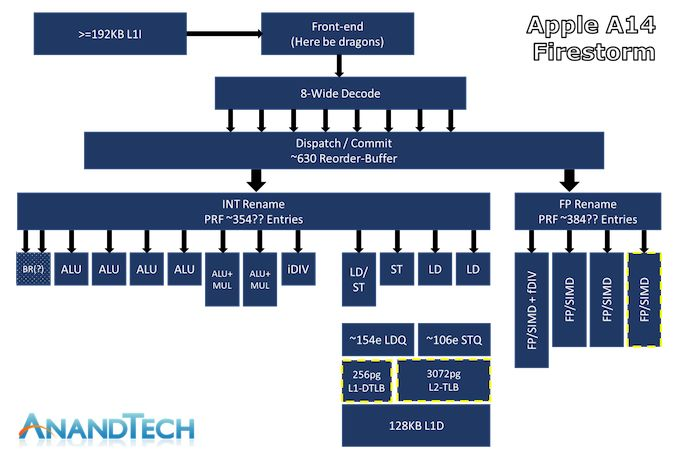
\includegraphics[width=\textwidth]{arch.jpg}

\subsubsection{对比和分析}

% Please add the following required packages to your document preamble:
% \usepackage{graphicx}
\begin{table}[]
  \centering
  \resizebox{\textwidth}{!}{%
    \begin{tabular}{|l|l|l|l|l|l|l|l|l|l|}
      \hline
      CPU          & A13-Ligthning & A14-FireStorm & Cortex-A77 & Cortex-A78 & Cortex-X1 & Zen2   & Zen3   & Skylake & Sunny Cove \\ \hline
      L1l(KiB)     & 128           & 192           & 64         & 32/64      & 64        & 32     & 32     & 32      & 32         \\ \hline
      L1D(KiB)     & 128           & 128           & 64         & 32/64      & 64        & 32     & 32     & 32      & 48         \\ \hline
      L2(MiB)      & 8             & 12            & 0.25/0.5   & 0.25/0.5   & 1         & 0.5    & 0.5    & 0.25    & 0.5        \\ \hline
      解码宽度     & 7             & 8             & 4          & 4          & 5         & 4      & 4      & 5       & 5          \\ \hline
      ROB          &               & 630           & 160        & 160        & 224       & 224    & 256    & 224     & 352        \\ \hline
      Int Reg File &               & 354           &            &            &           & 180    & 192    & 180     &            \\ \hline
      FP Reg File  &               & 384           &            &            &           & 160    & 160    & 168     &            \\ \hline
      ALU          &               & 6             & 3          & 4          & 4         & 4      & 4      & 4       & 4          \\ \hline
      FPU          &               & 128bx4        & 128bx2     & 128bx2     & 128bx4    & 256bx2 & 256bx2 & 256bx2  & 256bx3     \\ \hline
    \end{tabular}%
  }
  \caption{架构对比}
  \label{tab:1}
\end{table}

从表\ref{tab:1}中可以看到,最重要的执行单元部分,M1 / A14 的 6 个 ALU ,4 个 FPU 带来的最高理论性能直接就比其它 CPU 高 50\% ~ 100\%(暂不考虑 x86 256bit 的 AVX )。而 M1 的 L1 / L2 容量、解码宽度、ROB 规模都非常大,往往是其它 CPU 的两三倍(其中 12 MiB 的 L2 容量是四个大核共享,平均 3  MiB / 核心,但运行单线程应用的时候,理论上可以全部由单个核心使用),前端、调度单元、缓存的庞大规模,保证了执行单元能最高效率发挥性能。
所以,不考虑更多细节的话,假设大家性能效率发挥基本一致,理论上 M1 的 IPC ,整数方面应该比 Zen 2 / 3、SKL、SNC 都高50\%;不考虑 AVX ,浮点方面比Zen 2 / 3、SKL / SNC高 100\%。而 x86 的高频率所必须的长流水线,在分支预测失败需要重新填充流水线的时候,惩罚会比 M1 高,所以实际 IPC 要更低些;Intel 家的 FPU 和 ALU 共享发射端口,IPC 可能会更低一点。

解码器部分,x86 的变长指令解码器需要解析完一条指令得知本条指令长度后,才能计算出下一条指令的起始地址;在此之前,CPU 无法知道下一条指令从哪里开始,对连续的指令序列无法分拆后并行解码。虽然程序中会有类似跳转 (JMP)、调用 (CALL) 这样的分支指令,其操作数是某条指令的起始地址,另一个解码器可以从该地址开始解码,实现对指令序列进行并行解码。但毕竟程序中这样的指令密度有限,即便 CPU 中有更多的解码器对更多分支的指令并行解码,往往某个解码器解码后的 μOPs 在多个时钟周期内也不会进入执行序列。今天的 x86 CPU,AMD 已经是四个复杂解码器,Intel 是一个复杂解码器+四个简单解码器,已经有点过于富裕,这也是两家的CPU都支持 SMT (Simultaneous MultiThreading,同时多线程,也就是Intel的Hyper Thrading,超线程),并且开启 SMT 后多线程性能往往有相当幅度提升的一个重要原因,因为对两个线程并行解码后可以进入执行序列的 μOPs 数量更多。


而 RISC 的定长指令,指令抓取单元直接对指令序列按长度分割后,交由不同的解码器并行解码即可。因此可以看到两个超宽的 RISC 架构:IBM 最新的 POWER 可以配置为支持 SMT8,以及虽然不支持 SMT 但 IPC 惊人的苹果 A 系列。在 CISC 的 x86 上则没有出现过类似的超宽架构。


\subsection{GPU}
M1 集成了 Apple 设计的 8 核(在某些基本型号中为七核)图形处理单元 (GPU)。每个 GPU 核心被分成 16 个执行单元,每个执行单元包含 8 个算术逻辑单元 (ALU)。 M1 GPU 总共包含多达 128 个执行单元或 1024 个 ALU,Apple 表示它们可以同时执行多达 24,576 个线程,其最大浮点 (FP32) 性能为 2.6 TFLOP。

M1 Pro 集成了 Apple 设计的 16 核(在某些基本型号中为 14 个)图形处理单元 (GPU),而 M1 Max 则集成了一个 32 核(在某些基本型号中为 24 个)GPU。每个 GPU 核心分为 16 个执行单元,每个执行单元包含 8 个算术逻辑单元 (ALU)。 M1 Max GPU 总共包含多达 512 个执行单元或 4096 个 ALU,其最大浮点 (FP32) 性能为 10.4 TFLOP。

\subsection{其他特性}
M1 在处理器所有组件共享的统一内存配置中使用 4,266 MT/s LPDDR4X SDRAM。 SoC 和 RAM 芯片以系统级封装设计安装在一起。提供 8 GB 和 16 GB 配置。

M1 在 16 核神经引擎中包含专用的神经网络硬件,每秒能够执行 11 万亿次操作。其他组件包括图像信号处理器 (ISP)、NVMe 存储控制器、Thunderbolt 4 控制器和 Secure Enclave。

支持的编解码器包括 H264 和 H265(8/10 位,最高 4:4:4)、VP9 和 JPEG。

\section{性能和效率}

M1 在流行的基准测试(Geekbench 5、Cinebench R23)中记录了具有竞争力的性能和效率。

配备 2020 M1 的 Mac mini 在空闲时消耗 7 瓦,在最大负载时消耗 39 瓦,而 2018 年 6 核 Intel i7 Mac mini 的空闲时为 20 瓦,最大负载为 122 瓦。 M1 的能效使基于 M1 的 MacBook 的电池寿命比之前基于英特尔的 MacBook 增加了一倍。

在发布时,MacBook Air(M1,2020)和 MacBook Pro(M1,2020)被认为是 Apple 生产的最快的 MacBook。

\subsection{Cinebench R23}

\subsection{GeekBench 5}


\section{参考文献}
参考文献\cite{quinn1994parallel}\cite{golub2014scientific}\cite{joseph2022parallel}
% \textbf{超链接}  \href{http://youtube.com/}{YouTube}

\newpage
\bibliographystyle{plain}
\bibliography{reference.bib}

\end{document}